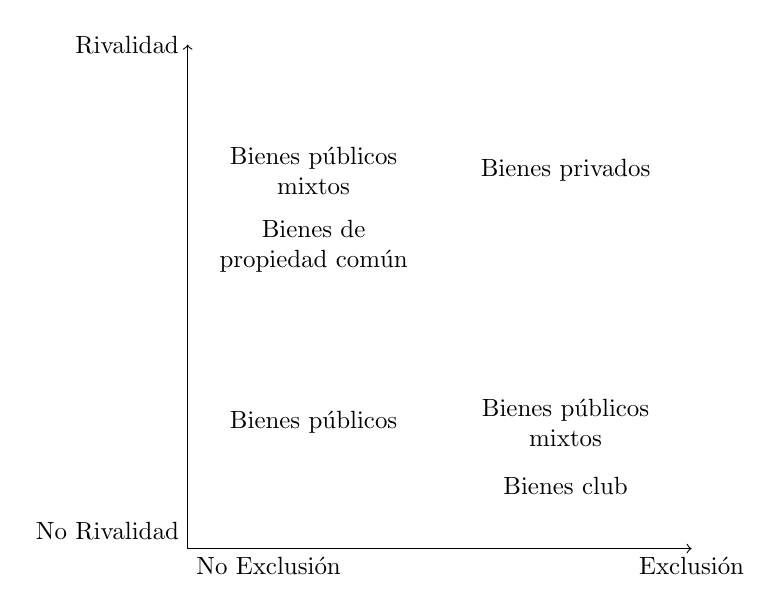
\begin{tikzpicture}[scale=0.8]
	\draw[<->] (0,8) node [left, scale=0.9] {Rivalidad} -- (0,0) -- (8,0) node [below, scale=0.9] {Exclusión};
	
	\draw (0,0) node [below right, scale=0.9] {No Exclusión};
	\draw (0,0) node [above left, scale=0.9] {No Rivalidad};
	
	\draw (2,6) node [text width=25mm,text centered, scale=0.9] {Bienes públicos mixtos};
	\draw (2,4.8) node [text width=30mm,text centered, scale=0.9] {Bienes de propiedad común};
	
	\draw (2,2) node [text width=25mm,text centered, scale=0.9] {Bienes públicos};
	
	\draw (6,2) node [text width=25mm,text centered, scale=0.9] {Bienes públicos mixtos};
	\draw (6,1) node [text width=25mm,text centered, scale=0.9] {Bienes club};
	
	\draw (6,6) node [text width=25mm,text centered, scale=0.9] {Bienes privados};
\end{tikzpicture}